\documentclass[11pt]{article}
\usepackage[margin=1.15in]{geometry}
\usepackage{amsmath,amssymb,amsthm}
\usepackage{booktabs}
\usepackage{graphicx}
\usepackage{microtype}
\usepackage[authoryear,round]{natbib}
\usepackage[colorlinks=true,linkcolor=black,citecolor=black,urlcolor=black]{hyperref}
\usepackage{setspace}
\onehalfspacing

\newtheorem{proposition}{Proposition}
\theoremstyle{definition}
\newtheorem{definition}{Definition}

\newcommand{\E}{\mathbb{E}}
\renewcommand{\Re}{\operatorname{Re}}

\title{A Proof of the Wrong Thing\\[4pt]
\large What a Verified Derivation Certifies and What It Leaves Open}
\author{Flyxion\\Independent Researcher}
\date{October 2026}

\begin{document}
\maketitle

\begin{abstract}
\noindent
Automated derivation and verification are being proposed as a way to establish mathematical results in wireless communications. A derivation that passes a symbolic or numerical check certifies a conditional statement: the conclusion follows from the stated model. Whether the conclusion answers the question a system designer asks depends on three further links that no checker of the derivation supplies: that the stated model is the one intended, that the quantity derived is the one that matters, and that the regime in which the result holds is the regime of use. This essay makes each link concrete with computations. A Cram\'er--Rao bound derived correctly under a known path gain is more optimistic than the unknown-gain bound by a factor that depends on an arbitrary choice of array index origin, a factor that equals one-quarter in the far-field limit and one when the index origin is moved to the array centre. A correct bound is not an attainable error, and the maximum-likelihood estimator in a simple example exceeds it by more than two orders of magnitude below a threshold signal-to-noise ratio. A capacity expression that is exact for independent Rayleigh fading overstates the capacity of a correlated channel by up to $4.9$ bit/s/Hz in a four-by-four example. Finally, the arithmetic of reporting the best of several runs and the sampling error of failure-mode percentages computed from a small number of failures are worked out. The target is the inference from ``verified'' to ``true of the system,'' not the verification itself, which is valuable for exactly what it certifies.
\end{abstract}

\section{A certificate has a domain}

A recent Perspective on formal mathematical reasoning for wireless communications \citep{zhao2026} proposes three layers: verification of established results, derivation of new ones, and discovery. Its case study asks language-model agents to derive Cram\'er--Rao bounds (CRBs) for sensing problems, using a symbolic engine, and checks the output against reference formulas and by numerical substitution. The Perspective is explicit about two things that matter here. First, the case study is scoped: it ``is not to test whether an LLM can formulate an ISAC sensing problem from scratch,'' and instead evaluates whether agents ``can execute and verify intermediate symbolic derivations under given wireless-domain models.'' Second, it argues that analytical systems should ``assess whether their assumptions and intermediate results remain valid under live deployment conditions.''

Both statements are correct and important. This essay takes the second as its subject and argues that it describes the central difficulty rather than a refinement. The reason is structural. Any checker, whether a proof assistant, a computer algebra system, or a numerical spot check, establishes a judgment of the form
\begin{equation}
\Gamma \vdash \varphi,
\label{eq:judgment}
\end{equation}
where $\Gamma$ collects the model and assumptions as they were formalized and $\varphi$ is the conclusion as it was formalized. The judgment is a statement about the formal objects. A reader who cites the result as a fact about a deployed system makes three further inferences, none of which is a theorem:
\begin{enumerate}
\item[(A)] \emph{Premise validity.} $\Gamma$ describes the system, so that the premises are true of it.
\item[(B)] \emph{Fidelity of the conclusion.} $\varphi$ is the quantity the reader means, so that its formal statement answers the question being asked.
\item[(C)] \emph{Regime.} The values of the parameters at which the conclusion is used lie inside the region where $\varphi$ is informative.
\end{enumerate}
The case study is designed so that $\Gamma$ and $\varphi$ are handed to the agents (the Perspective's Table~4 separates what is ``given in scenario'' from what must be derived), which is a legitimate design for testing symbolic execution. It also means that the conclusion drawn from its failure statistics, that the bottleneck ``lies not in understanding the task'' but in executing symbolic steps, is a statement about a task whose formulation was supplied. Section~\ref{sec:report} returns to this.

The following three sections isolate (A), (C) and (B) with computations on small, standard models. They are illustrations of the logical gap, not replications of the case study.

\section{Premise validity: a bound that depends on an index convention}

The near-field scenario in the Perspective's Table~4 has a uniform linear array with steering vector
\begin{equation}
[\mathbf a(R,\theta)]_m = \exp\!\Big[j\tfrac{2\pi}{\lambda}\Big(md\sin\theta-\tfrac{(md)^2\cos^2\theta}{2R}\Big)\Big],\qquad m=0,\dots,M-1,
\end{equation}
observation $\mathbf r=\alpha\,\mathbf a(R,\theta)s+\mathbf n$ with $\mathbf n\sim\mathcal{CN}(\mathbf 0,\sigma^2\mathbf I)$, $|\alpha|=1$, and Fisher information $F_{ij}=\tfrac{2|\alpha|^2}{\sigma^2}\Re\big[\tfrac{\partial\mathbf a^H}{\partial\eta_i}\tfrac{\partial\mathbf a}{\partial\eta_j}\big]$ for $\boldsymbol\eta=[\theta,R]^T$. The complex path gain $\alpha$ is part of the specification, with known modulus and, implicitly, known phase. A derivation that follows this model is correct if it returns the inverse of this $2\times2$ matrix. Nothing in the check can reveal that the model fixed a quantity that a receiver would normally have to estimate.

How much this matters can be computed. Let $\boldsymbol\eta$ be extended by the real and imaginary parts of $\alpha$, treated as unknown nuisance parameters. The Fisher matrix is then $4\times4$, and the CRB for $\theta$ is the corresponding entry of its inverse, which by the Schur complement is the known-gain information with the part explained by the nuisance directions removed.

\begin{proposition}
In the far-field limit with a single angle parameter, $\mathbf a_m=e^{j\pi m\sin\theta}$ and $m=0,\dots,M-1$, the ratio of the known-gain CRB to the unknown-complex-gain CRB for $\theta$ is
\begin{equation}
\frac{\mathrm{CRB}^{\mathrm{known}}_\theta}{\mathrm{CRB}^{\mathrm{unknown}}_\theta}
=1-\frac{(\sum_m m)^2}{M\sum_m m^2}=\frac{M+1}{2(2M-1)}\;\xrightarrow[M\to\infty]{}\;\tfrac14 .
\end{equation}
If the index origin is moved to the array centre, $m\mapsto m-(M-1)/2$, the ratio is exactly $1$.
\end{proposition}

\begin{proof}
The derivative $\partial_\theta\mathbf a$ equals $j\pi\cos\theta\,\mathrm{diag}(m)\,\mathbf a$. The nuisance directions are $\mathbf a$ and $j\mathbf a$. Because $\Re[\mathbf a^H\,j\,\mathrm{diag}(m)\mathbf a]=0$, only the $j\mathbf a$ direction couples to $\partial_\theta\mathbf a$, with inner product proportional to $\sum_m m$. The Schur complement removes the fraction $(\sum m)^2/(M\sum m^2)$ of the angle information, and with $\sum m=M(M-1)/2$ and $\sum m^2=(M-1)M(2M-1)/6$ the stated expression follows. Centering makes $\sum m=0$, so the coupling vanishes.
\end{proof}

The same bound is therefore three to four times smaller when the model fixes the gain at the first element than when the gain is unknown, and it is not smaller at all if the origin of the index is moved to the middle. Both known-gain bounds are correct derivations. They differ because knowing the gain at element zero fixes the carrier phase at one end of the aperture, and a phase known at one end constrains the slope of the phase across the aperture, which is the angle. When the phase is known at the centre instead, it carries no information about the slope. A property of the notation has been turned into a property of the physics.

Table~\ref{tab:crb} gives the values for the near-field model with both $\theta$ and $R$ unknown, computed by assembling the Fisher matrices numerically (wavelength $0.1$ m, spacing $\lambda/2$, $\theta=30^\circ$). The angle ratio is independent of $R$ to nine digits, because with $R$ free the even-order part of $\partial_\theta\mathbf a$ is absorbed by the range column, leaving the far-field structure. The range ratio is about one half whichever origin is used.

\begin{table}[h]
\centering
\caption{Known-gain CRB divided by unknown-complex-gain CRB, near-field ULA, $\theta=30^\circ$. Origin at the first element or at the array centre. The angle ratio does not depend on $R$ (checked at $R=3,10,30$ m).}
\label{tab:crb}
\begin{tabular}{rcccc}
\toprule
$M$ & $\theta$, first element & $\theta$, centre & $R$, first element ($R=10$ / $30$ m) & $R$, centre \\
\midrule
16 & 0.306 & 1.000 & 0.507 / 0.512 & 0.442 \\
32 & 0.277 & 1.000 & 0.463 / 0.474 & 0.444 \\
64 & 0.263 & 1.000 & 0.431 / 0.451 & 0.444 \\
\bottomrule
\end{tabular}
\end{table}

The lesson is not that the specified model is wrong. A known unit-modulus gain is a defensible modeling choice and the resulting bound answers a well-posed question, namely what is achievable with an oracle that supplies the gain. The lesson is that no check of the derivation distinguishes ``the bound for this system'' from ``the bound for this system plus an oracle whose value depends on a convention.'' That distinction lives in $\Gamma$, and the Perspective's closing recommendation, that nominal assumptions be tested against data, is exactly the process that would surface it. A formal library that is to support verification would need the assumption to appear in the statement of the theorem, as an explicit hypothesis on the gain, so that the consequence of relaxing it is a different theorem and not an unnoticed change of premise.

\section{Fidelity of the conclusion: a bound is not an attainable error}

The CRB is a lower bound on the variance of unbiased estimators. A correct derivation of it is a theorem. What the bound says about any estimator that can be built, at a given signal-to-noise ratio, is a separate matter. The classical threshold effect \citep[see][]{vantrees1968} is the failure of attainability when the likelihood has competing peaks.

An illustration uses the far-field model with $M=16$ elements, a single snapshot, true angle $20^\circ$, unknown complex gain, and the maximum-likelihood estimator over a grid of 6001 angles. The CRB with unknown complex gain at $\sigma^2$ is computed from the $3\times3$ Fisher matrix. Table~\ref{tab:thr} compares it with the Monte Carlo mean squared error from 3000 trials per SNR.

\begin{table}[h]
\centering
\caption{Single-snapshot angle estimation, $M=16$, $\theta=20^\circ$. Mean squared error of the grid ML estimator against the CRB (3000 trials per row; at high SNR the ratio fluctuates by a few percent around one).}
\label{tab:thr}
\begin{tabular}{rccc}
\toprule
SNR (dB) & MSE (rad$^2$) & CRB (rad$^2$) & MSE / CRB \\
\midrule
$-10$ & $4.3\times10^{-1}$ & $1.7\times10^{-3}$ & 257 \\
$-5$ & $1.5\times10^{-1}$ & $5.3\times10^{-4}$ & 285 \\
$0$ & $2.2\times10^{-3}$ & $1.7\times10^{-4}$ & 13 \\
$5$ & $5.2\times10^{-5}$ & $5.3\times10^{-5}$ & 0.98 \\
$10$ & $1.7\times10^{-5}$ & $1.7\times10^{-5}$ & 1.02 \\
$20$ & $1.7\times10^{-6}$ & $1.7\times10^{-6}$ & 0.99 \\
\bottomrule
\end{tabular}
\end{table}

Above about $5$ dB the bound is attained to within sampling error. At $0$ dB the estimator is thirteen times worse than the bound, and at $-5$ dB and below the error saturates at the scale of the prior interval, so the bound is off by more than two orders of magnitude. The derivation of the bound is identical at every row and equally correct. A sensing system quoting the bound as its accuracy is right at $10$ dB and wrong by a factor of 13 at $0$ dB, and the verification certificate does not change between the rows.

The Perspective's case study scope covers the derivation of the bound, not claims about estimator performance, so this is not a deficiency of the case study. It illustrates why a verified conclusion needs a statement of the regime in which it is used: $\varphi$ in \eqref{eq:judgment} is ``the Fisher information inverse is $X$,'' and the reader's question is ``how accurately can this system localize at $0$ dB.'' Those coincide only above a threshold that is itself a theorem-sized object, and the library of verified results would have to carry it as a hypothesis or a companion result.

\begin{figure}[h]
\centering
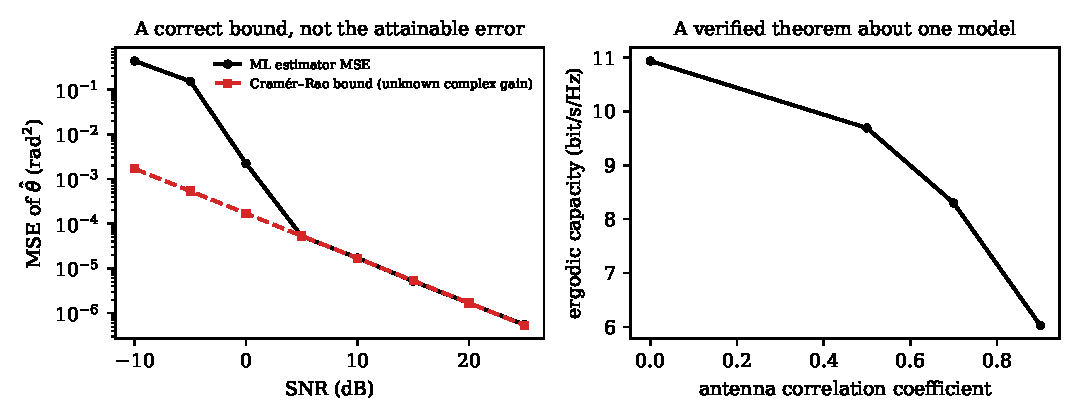
\includegraphics[width=\textwidth]{fig_wireless.pdf}
\caption{Left: ML angle-estimation error against the CRB for the model of Table~\ref{tab:thr}. Right: ergodic capacity of a $4\times4$ channel at $10$ dB under Kronecker exponential correlation (Table~\ref{tab:cap}).}
\label{fig:wireless}
\end{figure}

\section{Regime: an exact theorem about one model}

The Perspective cites the ergodic capacity expression
\begin{equation}
C=\E\log_2\det\!\Big(\mathbf I_{n_r}+\tfrac{\rho}{n_t}\mathbf H\mathbf H^H\Big)
\end{equation}
for an $n_r\times n_t$ channel with independent identically distributed Rayleigh fading, attributed to \citet{telatar1999}. The expression is exact and a formal derivation of it is a worthwhile target. What it certifies is capacity for the i.i.d.\ model. Real arrays are correlated, and the same expression with $\mathbf H$ replaced by $\mathbf R_r^{1/2}\mathbf G\mathbf R_t^{1/2}$ describes a different channel whose capacity is smaller \citep[the dependence of capacity on correlation is analyzed in][]{chuah2002}.

The size of the difference is easy to compute. Table~\ref{tab:cap} uses $n_t=n_r=4$, $\rho=10$ dB, and exponential correlation matrices $[\mathbf R]_{ik}=r^{|i-k|}$ at both ends, with $40{,}000$ channel draws per row.

\begin{table}[h]
\centering
\caption{Ergodic capacity of a $4\times4$ channel at $10$ dB, Kronecker exponential correlation with coefficient $r$ at both ends ($r=0$ is the i.i.d.\ case).}
\label{tab:cap}
\begin{tabular}{rcc}
\toprule
$r$ & capacity (bit/s/Hz) & shortfall relative to i.i.d. \\
\midrule
0.0 & 10.93 & 0 \\
0.5 & 9.69 & 1.24 \\
0.7 & 8.30 & 2.63 \\
0.9 & 6.03 & 4.91 \\
\bottomrule
\end{tabular}
\end{table}

At $r=0.9$ the i.i.d.\ expression overstates the capacity by $4.9$ bit/s/Hz, about $45\%$ of its value. The theorem is not wrong, and a machine-checked proof of it would be exactly as valid as before. The error is in applying it outside its model. Two features make this failure hard to catch from inside the formal system. First, the premise (i.i.d.\ entries) is a property of the channel distribution, which no proof about the expression can inspect. Second, asymptotic statements add a further, quieter regime: a result of the form $C=n\,c(\rho)+O(1)$ as $n$ grows is a statement about a limit, and the implied constant in $O(1)$ is part of the content that matters at $n=4$. A formalization that records the asymptotic claim without the constant certifies something true and, at the dimensions of interest, nearly empty.

A formal library built for use would state the capacity theorem for a family of covariance structures, so that the i.i.d.\ case is the instance $\mathbf R_t=\mathbf R_r=\mathbf I$ and a reader applying it to a measured channel must supply the covariance and see what changes. Doing so converts premise (A) from an unstated assumption to an input.

\section{What the case study's own statistics support}
\label{sec:report}

The Perspective reports, for each model and scenario, ``the best result over five independent runs.'' The design is reasonable for a study of what a model can do at all. It should not be read as the rate at which a single invocation succeeds. If a single run succeeds with probability $p$ independently, the best of five succeeds with probability $1-(1-p)^5$.

\begin{table}[h]
\centering
\caption{Probability that at least one of five independent runs succeeds, as a function of the single-run success probability $p$.}
\label{tab:best}
\begin{tabular}{rccccccc}
\toprule
$p$ & 0.1 & 0.2 & 0.3 & 0.4 & 0.5 & 0.6 & 0.8 \\
$1-(1-p)^5$ & 0.41 & 0.67 & 0.83 & 0.92 & 0.97 & 0.99 & 1.00 \\
\bottomrule
\end{tabular}
\end{table}

A scenario solved ``at best'' may therefore be solved one time in three, or one time in ten. In a deployment where a derivation is run once and relied upon, the relevant quantity is $p$, and the study as reported does not identify it. The text does state that DeepSeek-R1 solves all evaluated scenarios without Patcher revisions, which is a more favorable observation than best-of-five alone, but the per-run frequency is still not in the reported summary. This is a presentation point and not a flaw in the work: it is a statement of what the figure measures.

The same caution applies to the failure-mode breakdown. The percentages in the figure (29.4, 23.5, 23.5, 11.8, 5.9, 5.9) are all multiples of $1/17$, which is consistent with a total of 17 failures. On that reading, the categories correspond to $5,4,4,2,1,1$ events. Exact binomial 95\% intervals for the proportions are wide: $5/17$ has the interval $[0.10,0.56]$, $4/17$ has $[0.07,0.50]$, and $2/17$ has $[0.01,0.36]$. The ordering of the categories is not resolved by 17 events, and a category of two events cannot be distinguished from one of five. The finding that errors are predominantly algebraic rather than formulation errors may reflect agents that understand the task, or a benchmark that supplies the model; the counts alone cannot separate the two readings, and Section~1 explains why the design favors the second. Two items the text does not state are whether failures are counted over all runs or only over the selected best runs, and whether models are pooled, both of which change the denominator.

\section{What follows}

None of the above argues against machine-checked or machine-executed derivation. A derivation that passes a symbolic check is free of the algebraic slips that the case study identifies as the dominant failure, and for a long, error-prone derivation this is a real contribution. The argument concerns what to do with the certificate.

\paragraph{Make premises part of the statement.} Every example above is a case in which a hypothesis (known gain, i.i.d.\ entries, above-threshold SNR, large dimension) sat outside the theorem. If the library encodes each as an explicit argument, then a user must supply it, and the consequence of changing it is a recomputation, not an oversight. The Perspective's call for machine-readable formalization of wireless mathematics is the right place for this discipline.

\paragraph{Distinguish bounds from performance.} A verified bound should be tagged as a bound, with the conditions under which an estimator attains it recorded or marked as unknown.

\paragraph{Report single-run frequencies.} For benchmarks of derivation agents, the success rate of a single invocation, with an interval, answers the question that a user relying on one run asks. Best-of-$k$ is informative as a capability ceiling and should be labeled as such.

\paragraph{Test the premises against data.} The Perspective's own proposal of coupling derivations to digital-twin data streams is the right mechanism for premise validity. What the examples show is how large the stakes are: a factor of three to four in an angle bound from a convention, a factor over a hundred from a regime, and $45\%$ of capacity from a covariance assumption.

A proof of the right statement about the wrong model is still a proof, and the lesson of each example is that the wrongness was not in the proof.

\begin{thebibliography}{9}
\bibitem[Chuah et~al.(2002)]{chuah2002} Chuah, C.-N., Tse, D.~N.~C., Kahn, J.~M., Valenzuela, R.~A. (2002). Capacity scaling in MIMO wireless systems under correlated fading. \emph{IEEE Transactions on Information Theory} 48(3), 637--650.
\bibitem[Telatar(1999)]{telatar1999} Telatar, E. (1999). Capacity of multi-antenna Gaussian channels. \emph{European Transactions on Telecommunications} 10(6), 585--595.
\bibitem[Van Trees(1968)]{vantrees1968} Van Trees, H.~L. (1968). \emph{Detection, Estimation, and Modulation Theory, Part I}. Wiley.
\bibitem[Zhao et~al.(2026)]{zhao2026} Zhao, C., Wang, J., Niyato, D., Li, Z., Jamalipour, A., Wang, X., Kim, D.~I. (2026). Rethinking wireless communications through formal mathematical AI reasoning. \emph{npj Wireless Technology} 2, 81. doi:10.1038/s44459-026-00090-7.
\end{thebibliography}

\end{document}
